\subsubsection{Module de paramétrage}
\begin{figure}[h!]  
  \centering
    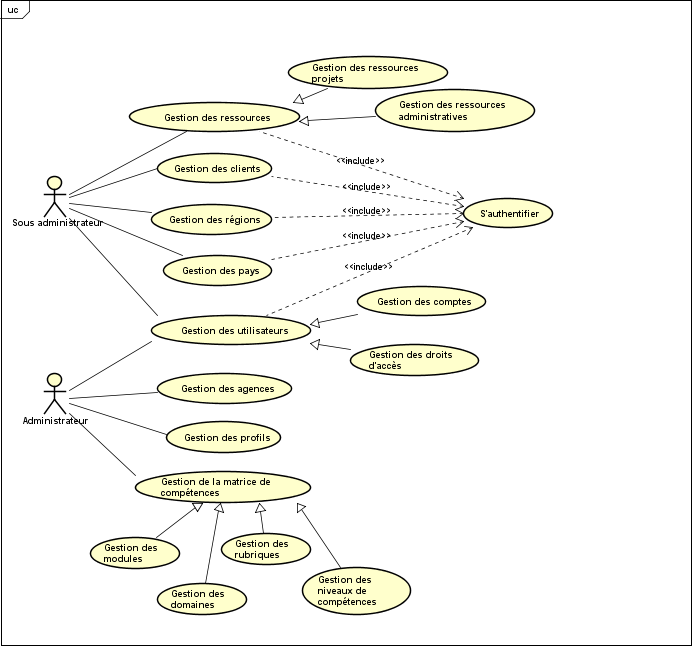
\includegraphics[width=0.95\textwidth]{chapitre2/Figures/parametrageUC.png}
  \caption{Diagramme de cas d’utilisation du module paramétrage}
\end{figure}
\newpage
\subsubsection*{Description des cas d’utilisations }
\begin{itemize}[label=\textbullet]
%Gestion des actions demandées
\item \textbf{Gestion des actions demandées :}
\begin{table}[!h]
\begin{tabular}{|p{15cm}|}%p{2.5cm}|p{9cm}
\rowcolor{shadecolor}\multicolumn{1}{|c|}{Sommaire d’indentification} \\
\hline
\textbf{objectif : } cette fonctionnalité permet de gérer les actions demandées\\
\textbf{acteurs : } administrateur\\
\textbf{précondition : } l'acteur est connecté au système\\
\hline
\rowcolor{shadecolor}\multicolumn{1}{|c|}{Description des scénarios} \\
\hline
	\textbf{Scénario nominal :}
	\begin{itemize}[label=\textbullet]
	\item scénario "ajouter action" :
		\begin{itemize}
		\item l'acteur ouvre le formulaire d'ajout
		\item l'acteur saisie les champs de l'action'
		\item l'acteur confirme l'ajout
		\item le système enregistre les données
		\end{itemize}
	\item scénario "modifier action" :
		\begin{itemize}
		\item l'acteur affiche la liste des actions
		\item l'acteur sélectionne l'action à modifier
		\item le système affiche les informations de l'action sélectionnée
		\item l'acteur modifie les champs ciblés
		\item l'acteur valide ses modifications
		\item le système confirme la modification
		\end{itemize}
	\item scénario "supprimer action" :
		\begin{itemize}
		\item l'acteur affiche la liste des actions
		\item l'acteur sélectionne l'action à supprimer
		\item le système affiche un message de confirmation
		\item l'acteur confirme la suppression
		\item le système supprime l'action'
		\end{itemize}
	\end{itemize}
	\textbf{Scénario Alternatives  :}\\
	Le système vérifie si l'action existe déjà dans la BD avant l’ajout.\\
\hline
\end{tabular}
\centering \caption{Description du cas d’utilisation "Gestion des actions demandées"} \label{TablePR}
\end{table}
%Gestion des états d'action
\newpage
\item \textbf{Gestion des états d'action :}\\
\begin{table}[!h]
\begin{tabular}{|p{15cm}|}%p{2.5cm}|p{9cm}
\rowcolor{shadecolor}\multicolumn{1}{|c|}{Sommaire d’indentification} \\
\hline
\textbf{objectif : } cette fonctionnalité permet de gérer les états d'action\\
\textbf{acteurs : } administrateur\\
\textbf{précondition : } l'acteur est connecté au système\\
\hline
\rowcolor{shadecolor}\multicolumn{1}{|c|}{Description des scénarios} \\
\hline
	\textbf{Scénario nominal :}
	\begin{itemize}[label=\textbullet]
	\item scénario "ajouter état" :
		\begin{itemize}
		\item l'acteur ouvre le formulaire d'ajout
		\item l'acteur saisie les champs d'état
		\item l'acteur confirme l'ajout
		\item le système enregistre les données
		\end{itemize}
	\item scénario "modifier état" :
		\begin{itemize}
		\item l'acteur affiche la liste des états
		\item l'acteur sélectionne l'état à modifier
		\item le système affiche les informations d'état sélectionnée
		\item l'acteur modifie les champs ciblés
		\item l'acteur valide ses modifications
		\item le système confirme la modification
		\end{itemize}
	\item scénario "supprimer état" :
		\begin{itemize}
		\item l'acteur affiche la liste des états
		\item l'acteur sélectionne l'état à supprimer
		\item le système affiche un message de confirmation
		\item l'acteur confirme la suppression
		\item le système supprime l'état
		\end{itemize}
	\end{itemize}
	\textbf{Scénario Alternatives  :}\\
	Le système vérifie si l'état existe déjà dans la BD avant l’ajout.\\
\hline
\end{tabular}
\centering \caption{Description du cas d’utilisation "Gestion des états d'action"} \label{TablePR}
\end{table}

%Gestion des états des composants
\newpage
\item \textbf{Gestion des états des composants :}\\
\begin{table}[!h]
\begin{tabular}{|p{15cm}|}%p{2.5cm}|p{9cm}
\rowcolor{shadecolor}\multicolumn{1}{|c|}{Sommaire d’indentification} \\
\hline
\textbf{objectif : } cette fonctionnalité permet de gérer les états des composants\\
\textbf{acteurs : } administrateur\\
\textbf{précondition : } l'acteur est connecté au système\\
\hline
\rowcolor{shadecolor}\multicolumn{1}{|c|}{Description des scénarios} \\
\hline
	\textbf{Scénario nominal :}
	\begin{itemize}[label=\textbullet]
	\item scénario "ajouter état" :
		\begin{itemize}
		\item l'acteur ouvre le formulaire d'ajout
		\item l'acteur saisie les champs d'état
		\item l'acteur confirme l'ajout
		\item le système enregistre les données
		\end{itemize}
	\item scénario "modifier état" :
		\begin{itemize}
		\item l'acteur affiche la liste des états
		\item l'acteur sélectionne l'état à modifier
		\item le système affiche les informations d'état sélectionnée
		\item l'acteur modifie les champs ciblés
		\item l'acteur valide ses modifications
		\item le système confirme la modification
		\end{itemize}
	\item scénario "supprimer état" :
		\begin{itemize}
		\item l'acteur affiche la liste des états
		\item l'acteur sélectionne l'état à supprimer
		\item le système affiche un message de confirmation
		\item l'acteur confirme la suppression
		\item le système supprime l'état
		\end{itemize}
	\end{itemize}
	\textbf{Scénario Alternatives  :}\\
	Le système vérifie si l'état existe déjà dans la BD avant l’ajout.\\
\hline
\end{tabular}
\centering \caption{Description du cas d’utilisation "Gestion des états des composants"} \label{TablePR}
\end{table}


\end{itemize}